\chapter{Overall Description}

\section{Product Perspective}

CSAF serves the role of a middleware to create closed loop system simulations. A user starts with a model that they have for a dynamical system, with well-defined input, outputs and states. Shown in Figure \ref{fig:ccomp}, they will proceed to create a CSAF compatible component. The package comes with an API to make common system descriptions easy to implement, and has a wrappers if the system is more of a black box. The outcome is a system that has a subscriber to collect input and a publisher to broadcast output. \\

\begin{figure}
\centering
\includegraphics[width=0.9\textwidth]{componentcomposition.pdf}
\caption{Structure of a CSAF Compatible Component}
\label{fig:ccomp}
\end{figure}

A CSAF component is intended to represent a plant or a controller, but not closed loop system. These components can be composed together to create a closed loop dynamical system. Figure \ref{fig:csys} shows the blocks composed under a system analyzer. In the scope of controls research, this is the benefit of CSAF. Analyses can be created and performed on the modular CSAF components. \\

\begin{figure}
\centering
\includegraphics[width=0.9\textwidth]{systemanalysis.pdf}
\caption{Analyzer for Closed Loop System of CSAF Components }
\label{fig:csys}
\end{figure}


\section{Product Functions}

A user is able to

\begin{enumerate}
\item add model specifics of a dynamical system to create a compatible component
\item compose controllers together to make closed loop systems
\item simulate a closed loop systems efficiently
\item design custom analyses, and is supported with libraries and documentation
\end{enumerate}

Figure \ref{fig:uworkflow} shows the user workflow for a systems analysis, from start to finish. All blocks in the control diagram must exist as components. Then, the components are composed together to achieve the controlled system. The system is ready to be simulated or analyzed.

\begin{figure}
\centering
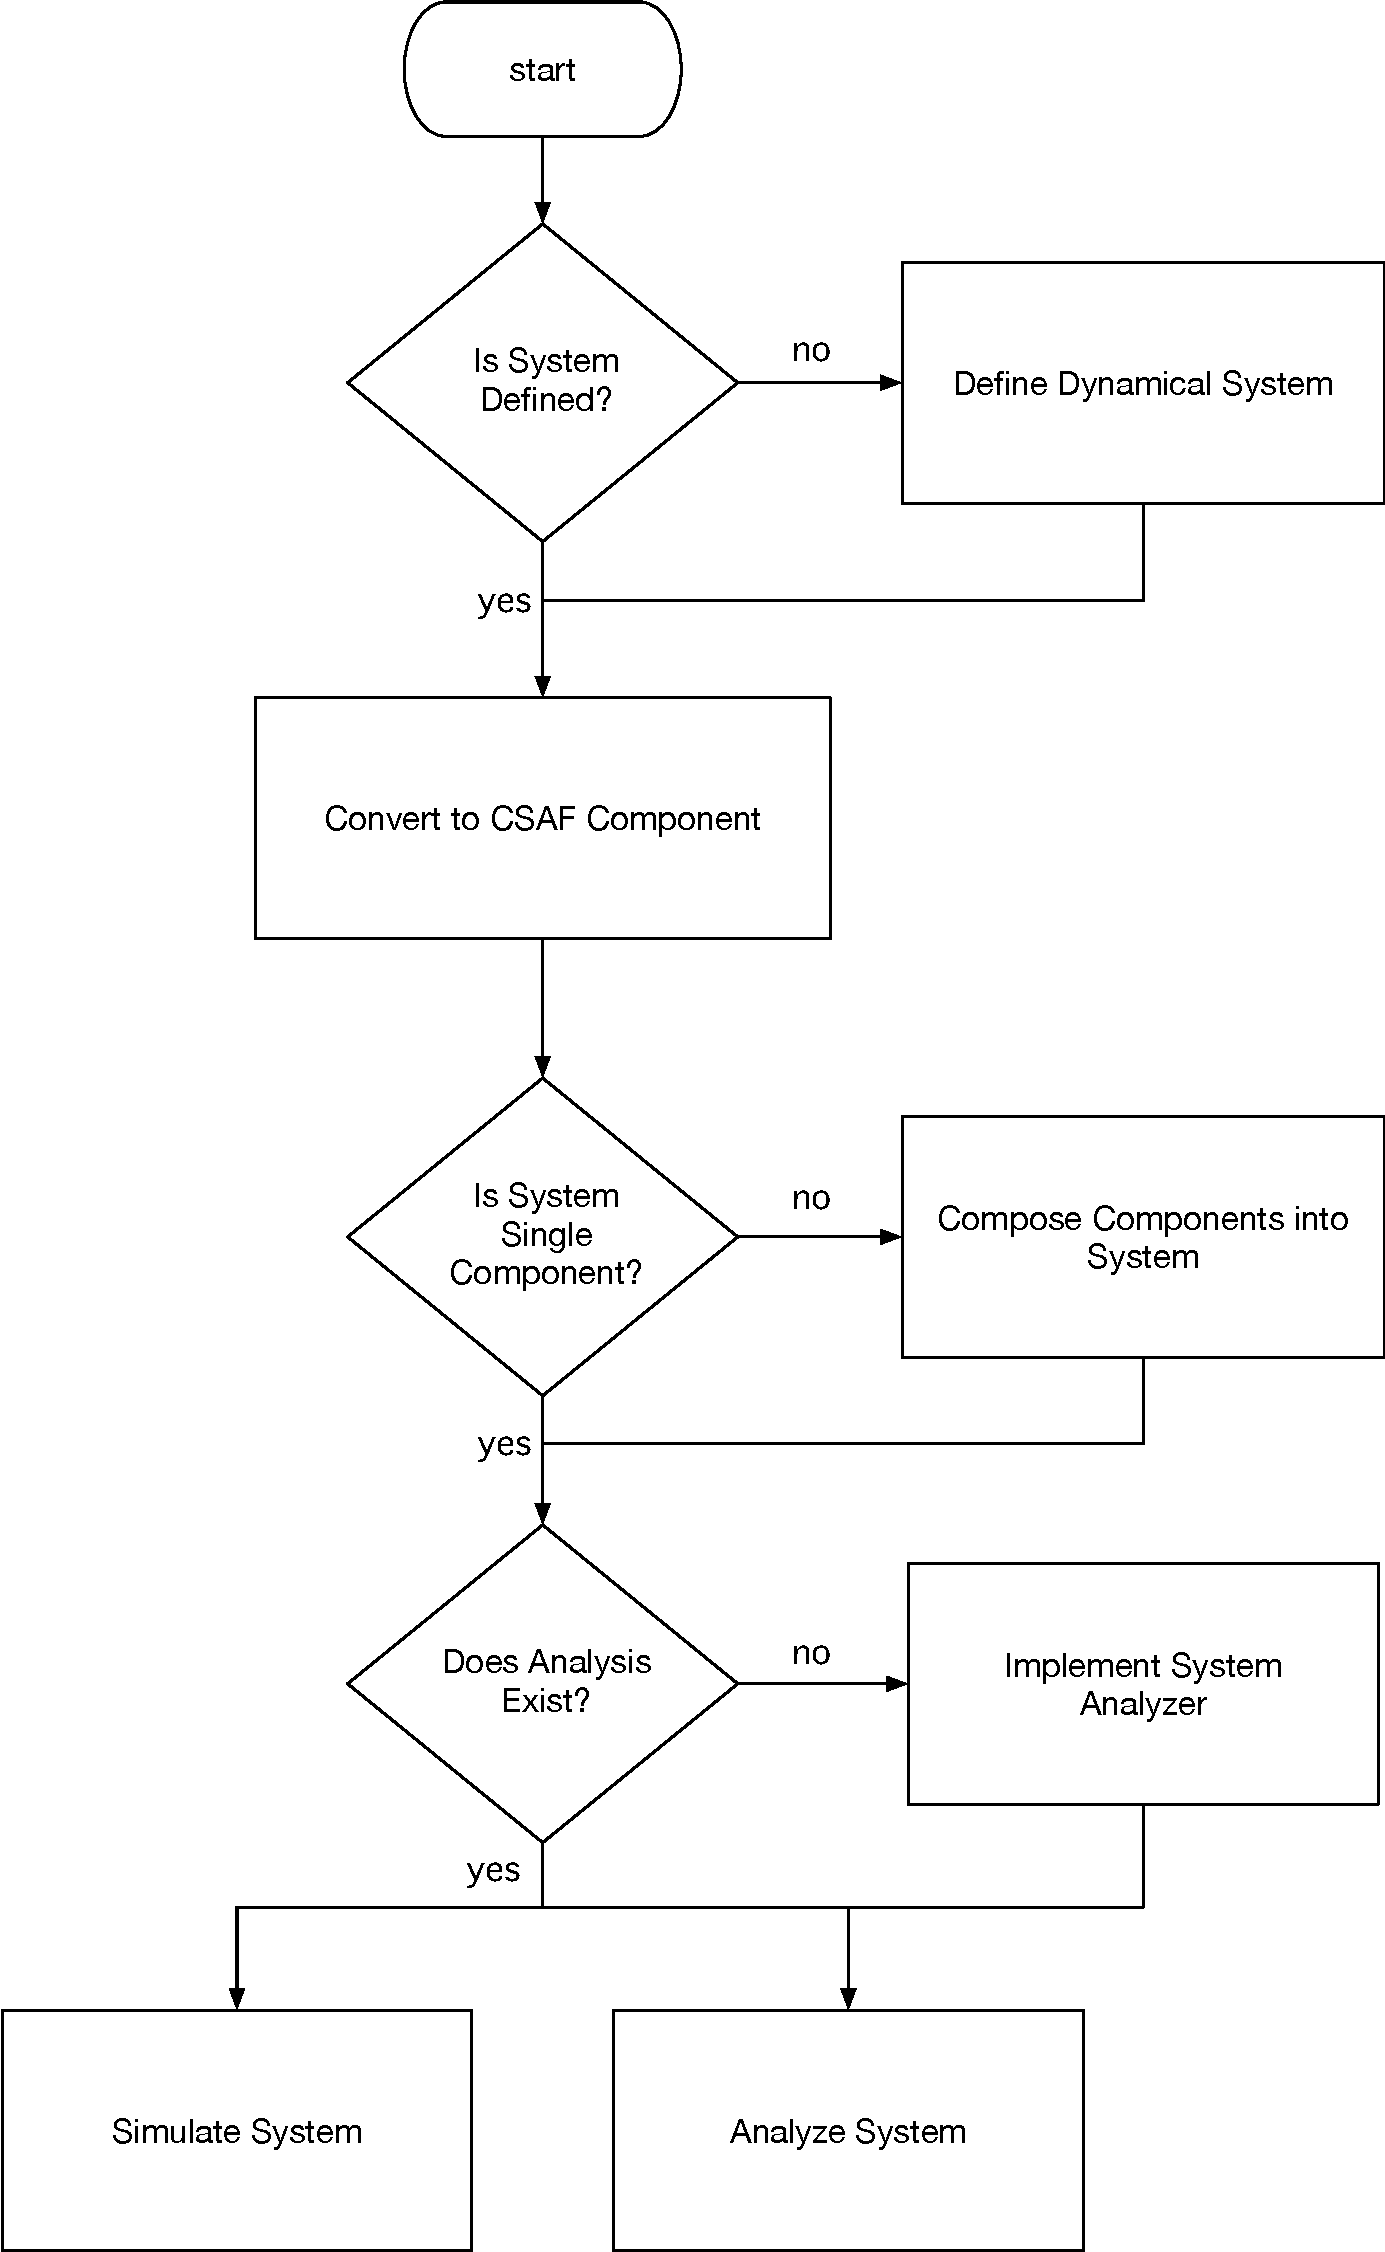
\includegraphics[width=0.85\textwidth]{userworkflow2.pdf}
\caption{ CSAF System Analysis User Workflow }
\label{fig:uworkflow}
\end{figure}

\section{User Classes and Characteristics}

CSAF's user workflow is restricted to software developers, systems engineers and researchers. The users implementing components are required to have substantial knowledge of programming and system theory. The workflow output is to provide results for a controls research project. As such, secondary users are project managers and reviewers. 


\section{Operating Environment}

CSAF is implemented in modern python (3.5+), with specific packages for numerical/controls computing. Also, it has optional package requirements, like tensorflow and RosPy needed for specific features. Its primary use is to operate inside a debian based docker container for its delivery in the Assured Autonomy project. For full use, it will require a OS with CoPilot installed, needing Haskell and C toolchains.  

\section{Design and Implementation Constraints}
$<$Describe any items or issues that will limit the options available to the 
developers. These might include: corporate or regulatory policies; hardware 
limitations (timing requirements, memory requirements); interfaces to other 
applications; specific technologies, tools, and databases to be used; parallel 
operations; language requirements; communications protocols; security 
considerations; design conventions or programming standards (for example, if the 
customer’s organization will be responsible for maintaining the delivered 
software).$>$

\section{User Documentation}

As CSAF users will need detailed knowledge of its architecture and API to use it effectively, documentation is important. Its code repository contain a number of markdown files that outline the installation and setup. For object and function level documentation, the code uses an ample amount of Python docstrings, which can be used to autogenerate API documentation if the code comments are suitably detailed. \\

API level documentation is not enough, and  a user manual is available. This manual is conscience of task oriented documentation; the workflow is discussed and examples are provided for intended implementation use. Further, the use cases are also described in Jupyter notebooks, which provide an interactive platform to experiment with code.

\section{Assumptions and Dependencies}

$<$List any assumed factors (as opposed to known facts) that could affect the 
requirements stated in the SRS. These could include third-party or commercial 
components that you plan to use, issues around the development or operating 
environment, or constraints. The project could be affected if these assumptions 
are incorrect, are not shared, or change. Also identify any dependencies the 
project has on external factors, such as software components that you intend to 
reuse from another project, unless they are already documented elsewhere (for 
example, in the vision and scope document or the project plan).$>$
